\section{Gesti�n de stock y productos}

Este componente se encarga de la gesti�n de los modelos correspondientes a
productos, tipos de procuto, insumos y las operaciones de alta y baja de los
mismos, as� como de las actualizaciones de sus valores.

Mediante la funcionalidad de ABM provista como se describe en \ref{metodosEstaticos}
es posible realizar los cambios necesarios al stock, tales como modificaciones de
precios o el ingreso de nuevos productos.

El Controlador de Stock es una entidad abstracta que se encarga de las modificaciones
de los valores de stock frente al ingreso o cancelaci�n de pedidos. Esta abstracci�n
se introduce para respetar DIP, y puesto que podr�a ser interesante brindar funcionalidad
m�s sofisticada en esta entidad. Por ejemplo, un controlador de stock m�s inteligente podr�a
realizar un seguimiento individual de todas las transacciones de stock llevadas a cabo
que permitir�a \textit{trackear} cada insumo.

El Controlador de Stock es responsable de emitir el evento de notificaci�n de stock
cr�tico, al que la GUI se suscribe para poder indicar al usuario que el stock requiere
de su atenci�n.

Las clases principales en lo que a modelos de datos respecta dentro de este componente
son Insumo y Producto. La clase TipoProducto permite reconocer cuando varios productos
tienen el mismo tipo y por tanto pueden tratarse de forma an�loga en cuanto a su
preparaci�n y cocci�n. 

El tipo de producto permite especificar adem�s si el producto es
cocinable o preparable. Si bien en el sistema actual los productos son ya sea preparable
y cocinables o ninguno de los dos, en el futuro la pizzer�a podr�a desear, por ejemplo,
comercializar ensaladas que solo requieren de preparaci�n y no de cocci�n. La existencia
de estos atributos permite flexibilidad adicional para extender la operatoria del
restaurante. Si bien esta elecci�n de atributos puede parecer limitante o arbitraria,
evaluamos que es factible categorizar de esta manera a cualquier tipo de producto
que podr�a venderse en una pizzer�a. Por lo tanto, no nos pareci� razonable agregar
complejidad al modelo agregando ``propiedades'' gen�ricas a los tipos de producto
(propiedades de las que \textit{cocinable} y \textit{preparable} ser�an un caso particular).

% TODO: hablar del repositorStock


\subsection{Modelado de escenarios}
\label{cosasDeStock}

% FIXME FIXME FIXME: todo esto tiene que volar, es cosa de la gesti�n de stock, no
% del ingreso de los pedidos, hay que moverlo y eventualmente rehacer estos diagramas
% pero sin tanto enfasis en el stock

El verificador de stock tiene por responsabilidad controlar que solo ingresen pedidos que puedan ser satisfechos. Ademas en caso de ser necesario debera notificar la existencia de insumos en stock critico.

Como vimos en el escenario de creaci�n de un pedido, el generador de pedidos invoca el metodo verificarEIngresar. Este metodo va a intentar decrementar el stock de los insumos de cada producto del pedido que se desea armar. Para eso va a decrementar el stock siempre que sea posible, guardando aquellos productos cuyos insumos ya modifico para poder hacer rollback en caso de que el pedido no se pueda satisfacer. Si ocurre que hay un insumo de un producto cuyo insumo es insuficiente, se procede a restablecer el stock ya decrementado y luego se genera un excepcion que permite que se pueda mostrar en pantalla cual fue el pedido que genero el error al intentar ingresar.

En cambio si todos los productos se pudieron ingresar, la funci�n retorna True para indicar que termino exitosamente. Notar que hay un problema de sintaxis en el diagrama, ya que se hace delete del multiconjuinto pero su linea de vida se extiende. Esto es porque el programa utilizado para los diagramas no soporta eliminar dos veces al mismo elemento (en verdad es solo una vez, ya que ambas no pueden ocurrir, pero no se da cuenta de eso).

\begin{figure}[H]
\centering
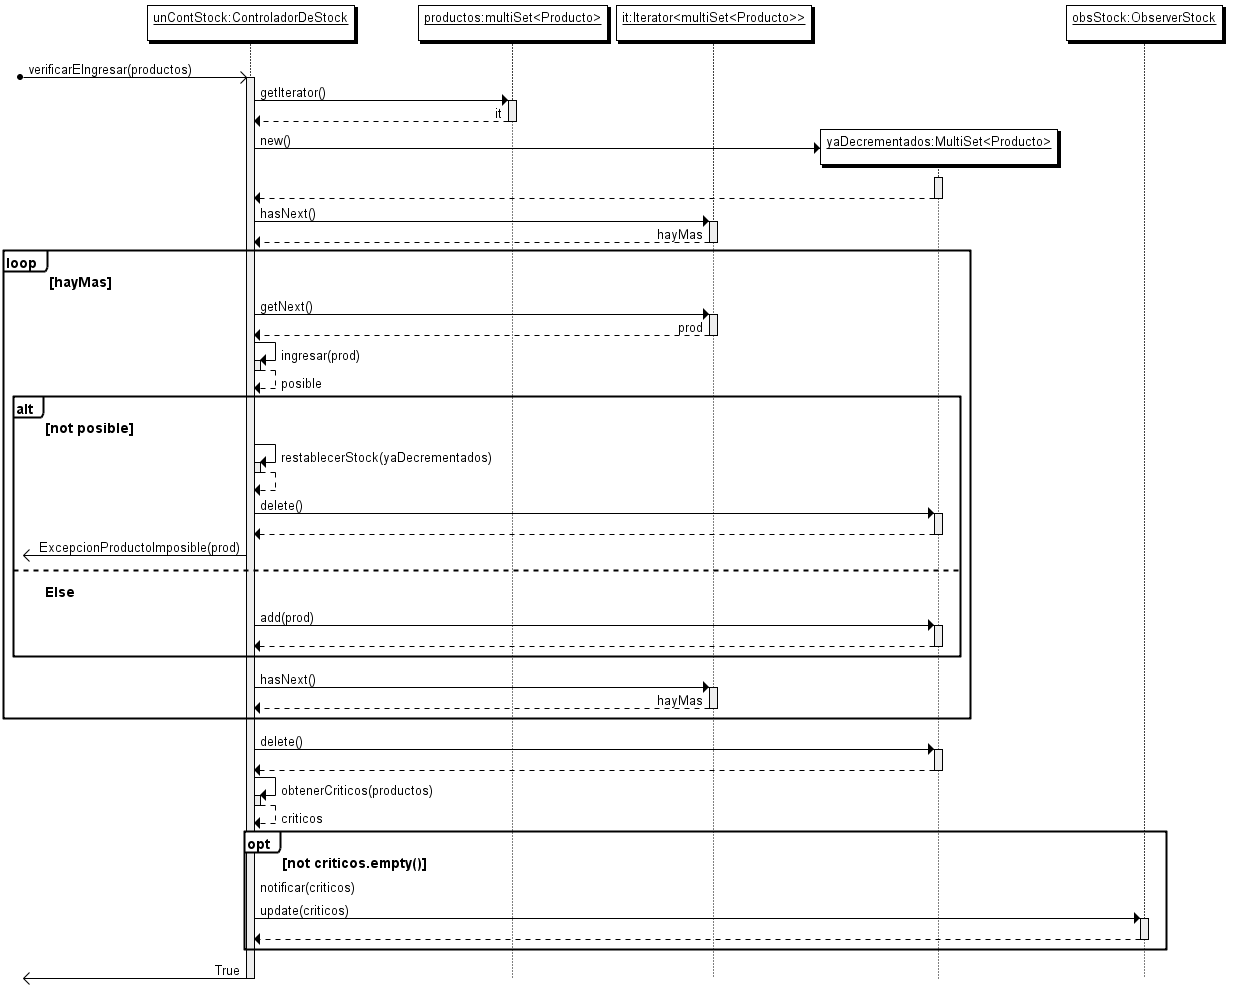
\includegraphics[height=15cm]{./figuras/verificarEIngresar.png}
\caption{Verificaci�n y decremento de stock de los insumos}
\end{figure}

Decidimos factorizar el diagrama de modo que algunas interacciones las mostraremos a continuaci�n. El metodo ingresar realiza la verificaci�n pero a nivel de cada producto, es decir revisa dado un producto que exista una cantidad de insumos necesaria. Al igual que el metodo anterior va recordando los stocks que ya modifico para hacer rollback en caso de que sea necesario.

\begin{figure}[H]
\centering
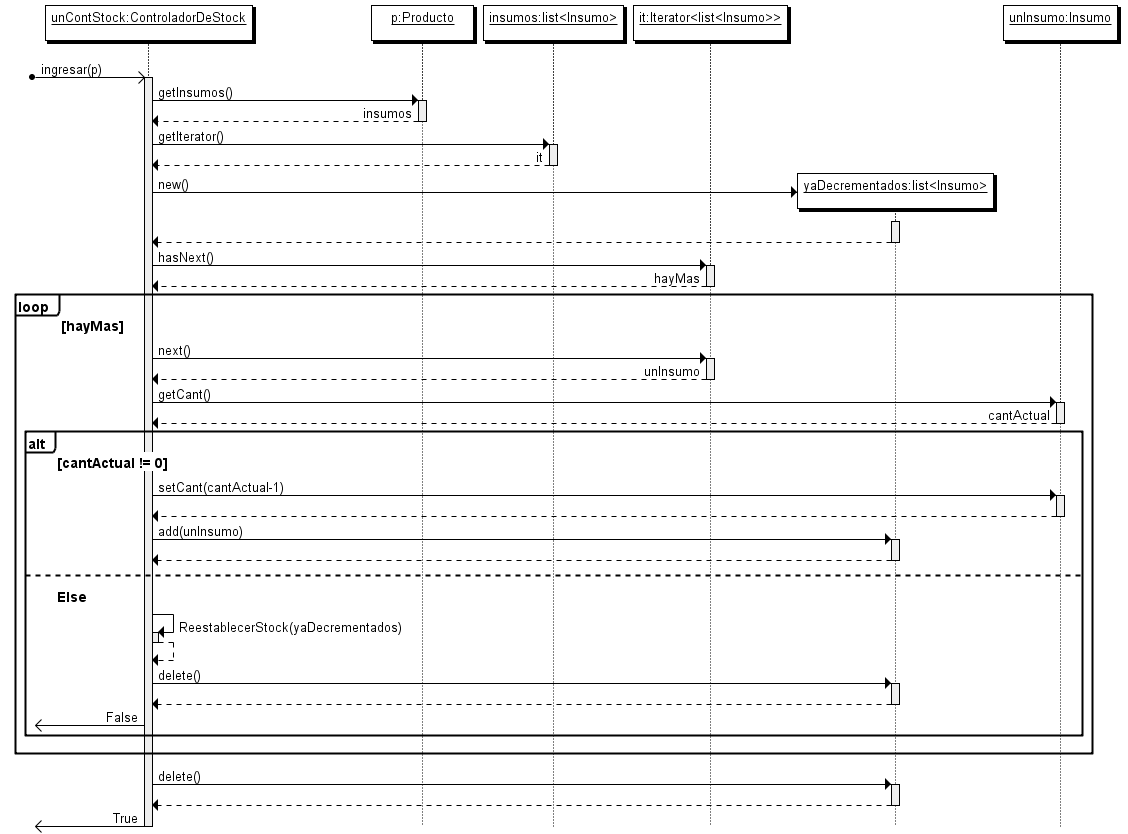
\includegraphics[height=11cm]{./figuras/ingresar(ControladorStock)}
\end{figure}

Hay dos metodos restablecerStock, uno trabaja sobre productos y otro a nivel de insumos. El primero recorre los productos llamando al segundo para los insumos de cada producto que itera. Mientras que a nivel de insumos, lo que se hace es incrementar la cantidad de cada insumo que aparece en la lista. Como dijimos anteriormente, estos metodos permiten realizar un rollback para deshacer los cambios hechos en el stock en el caso de que la operaci�n de ingreso no sea exitosa

\begin{figure}[H]
\centering
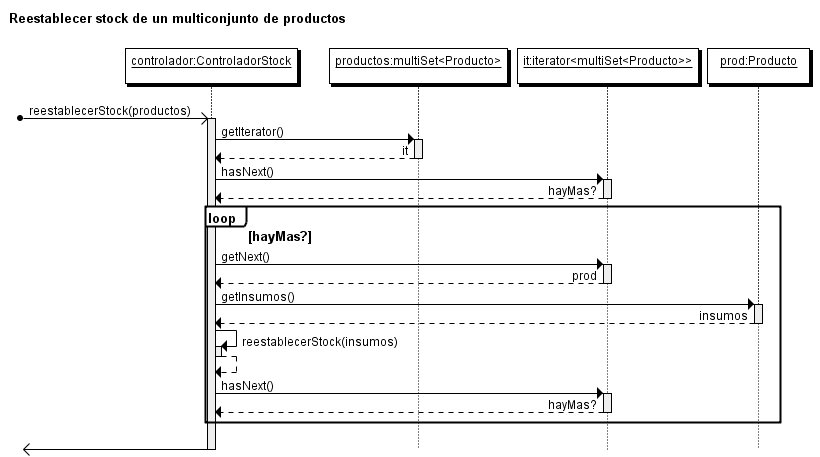
\includegraphics[height=9cm]{./figuras/reestablecerStockProductos}
\caption{restableciendo el stock de los productos cuyo stock se decremento }
\end{figure}

\begin{figure}[H]
\centering
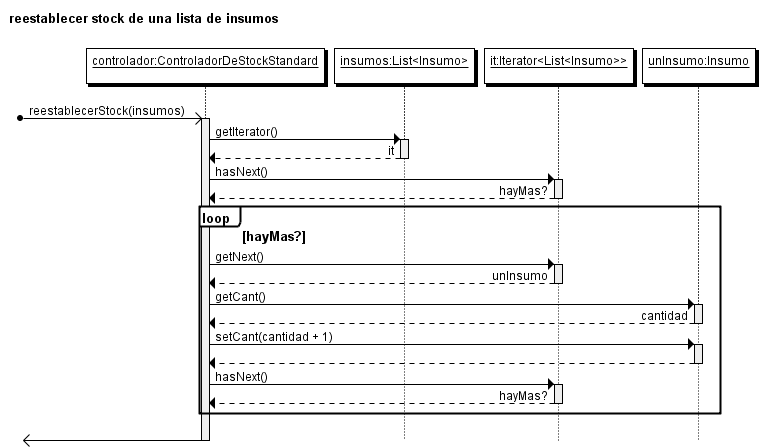
\includegraphics[height=9cm]{./figuras/reestablecerStockInsumos}
\caption{restableciendo el stock de los insumos que se decrementaron }
\end{figure}
% TODO: traer los diagramas de la parte de ingreso de pedidos

\textcolor{Red}{TODO: explicacion de metodos importantes}
% FIXME: vale la pena? creo que co los DS que estan en la parte de ingreso de pedidos alcanza y sobra
